%# -*- coding: utf-8-unix -*-
% !TEX program = xelatex
% !TEX root = ../thesis.tex
% !TEX encoding = UTF-8 Unicode
\chapter{需求分析}
在确认了系统基本可行之后,具体的系统设计和开发之前首要工作便是进行需求分析,
该阶段通过对用户的需求进行分析,识别和确认系统中的功能点,和所需达到的目标,
总结归纳得出系统的功能性和非功能性需求。
\section{功能性需求}
通过生活实际经验和网上对学生和白领群体对调查研究,总结的需求如下:
\begin{itemize}
	\item 自由添加、删除和修改任务信息
	\item 添加、删除和修改项目信息,并可以将任务添加入项目进行分类
	\item 同一项目中的任务可以选择依赖关系
	\item 一个需要多次完成的任务可以进行拆分,每次只完成其的一部分
	\item 通过任务预估时间计算空闲时间,并在适当位置给予提醒
	\item 通过任务的依赖关系计算合适的任务完成顺序,确保项目顺利推进
	\item 完成任务时记录当前任务完成时间和精力状态
	\item 根据以往的精力状态分配任务,并以图标的方式呈现
\end{itemize}

\begin{figure}[!htp]
	\centering
	\makebox[\textwidth]{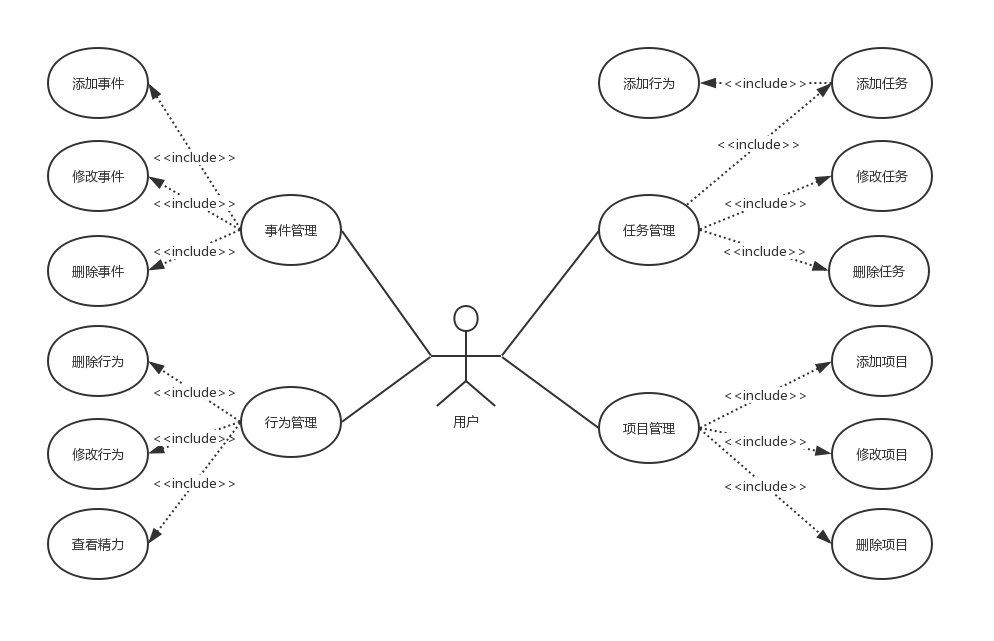
\includegraphics[width=\textwidth]{figure/uml/use_case.png}}
	\caption{任务计划及时间管理系统总用例图}
    \label{fig:use_case}
\end{figure}

图\ref{fig:use_case}基本包含了本系统的所有基本用例,
其中行为管理是根据需求分析得到的用于记录任务完成情况和精力分配的工具,
更为细致的用例描述见以下表格分析。

\begin{table}
	\centering
	\caption{用户添加任务用例描述表}
	\begin{tabular}{l|p{8cm}} \toprule
	  项目 & 内容说明 \\
	  \midrule
	  用例名称 & 用户添加任务 \\
	  参与者 & 用户 \\
	  前提条件 & 无 \\
	  前置操作 & 用户处于主界面状态 \\
	  后置操作 & 用户设置好任务信息后跳转回原界面 \\
	  合法流程 & 用户点击收件箱添加任务或长按收件箱添加任务,
	  设置好任务信息后点击保存 \\
	  异常情况举例 & 数据库或手机内部存储已满,无法添加 \\
	  \bottomrule
	\end{tabular}
\end{table}

\begin{table}
	\centering
	\caption{用户选择任务依赖关系用例描述表}
	\begin{tabular}{l|p{8cm}} \toprule
	  项目 & 内容说明 \\
	  \midrule
	  用例名称 & 用户选择任务依赖关系 \\
	  参与者 & 用户 \\
	  前提条件 & 用户已创建项目且项目中已含有任务 \\
	  前置操作 & 用户添加任务 \\
	  后置操作 & 跳转回添加任务界面 \\
	  合法流程 & 用户点击添加任务,选择合适的项目进行归类,
	  选择同一项目中的其他任务设置依赖关系 \\
	  异常情况举例 & 由于已经通过算法帮助用户排除了可能出现的
	  依赖关系形成环的情况,故在满足前提条件的情况下,基本无异常情况出现 \\
	  \bottomrule
	\end{tabular}
\end{table}

\begin{table}
	\centering
	\caption{用户完成任务用例描述表}
	\begin{tabular}{l|p{8cm}} \toprule
	  项目 & 内容说明 \\
	  \midrule
	  用例名称 & 用户选用户完成任务 \\
	  参与者 & 用户 \\
	  前提条件 & 用户已创建任务 \\
	  前置操作 & 用户添加任务 \\
	  后置操作 & 保持原界面或添加行为界面 \\
	  合法流程 & 用户点击完成任务,若任务未被分割,则直接完成,
	  若任务已被分割,则进入用户添加行为界面 \\
	  异常情况举例 & 数据库或手机内部存储已满,无法添加行为 \\
	  \bottomrule
	\end{tabular}
\end{table}

\begin{table}
	\centering
	\caption{用户添加事件用例描述表}
	\begin{tabular}{l|p{8cm}} \toprule
	  项目 & 内容说明 \\
	  \midrule
	  用例名称 & 用户添加事件 \\
	  参与者 & 用户 \\
	  前提条件 & 用户已授权系统日历使用权限 \\
	  前置操作 & 用户位于今日界面 \\
	  后置操作 & 保持原界面 \\
	  合法流程 & 用户未授权系统日历则弹出对话框授权使用,
	  若已授权则弹出添加事件的界面并进行设置 \\
	  异常情况举例 & 用户未授权系统日历,无法添加事件 \\
	  \bottomrule
	\end{tabular}
\end{table}

对于用户的需求进行分析后,发现任务这一实体的粒度不够细,需要再进行细化
也就是之前提到的行为,通过行为,我们可以更加细腻的了解用户在每个时间段的状态
便于以后的统计和分析,具体如图\ref{fig:activity}。

\begin{figure}
	\centering
	\makebox[\textwidth]{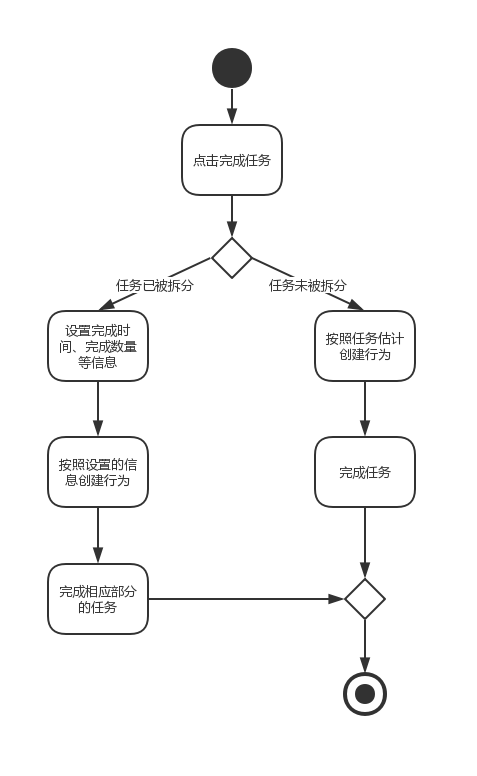
\includegraphics[height=12cm]{figure/uml/activity.png}}
	\caption{用户选择完成任务的活动图}
    \label{fig:activity}
\end{figure}

\section{其他需求}
\subsection{用户界面}
本系统的用户界面采用统一的GUI界面,并保持与iOS 系统应用风格的一致性,
其中出现的所有错误信息和提示信息均采用与系统风格统一的标准提示框。

\subsection{通讯接口}
\begin{itemize}
	\item 预留与Apple 服务器通讯并进行同步的iCloud 服务接口。
	\item 日常使用中可以不依赖网络使用,确保随时可用。
	\item 与其他日程管理类的软件通用接口:如系统日历,iCal通用日历信息文件。
	\item 与其他即时通讯类软件的交互接口:如文字信息入口等。
\end{itemize}

\subsection{性能需求}
\begin{itemize}
	\item 客户端一般响应时间不超过0.1秒。
	\item 任务统计时间不超过0.5秒。
\end{itemize}

\subsection{安全性需求}
\begin{itemize}
	\item 数据备份:允许用户进行数据的备份和恢复,以弥补数据的破坏和丢失。
	\item 加密:可以设置需要指纹或密码进入系统。
\end{itemize}

\subsection{可用性需求}
\begin{itemize}
	\item 控制必录入项:本系统能够对必须录入的内容进行控制,
	确保信息录入的完整。同时对必录入项进行有效的统一的提示,如使保存按钮不可用等。
	\item 容错能力:系统具有一定的容错和抗干扰能力,在非硬件故障或非通讯故障时,
	系统能够保证正常运行,并有足够的提示信息帮助用户有效正确地完成任务。
	\item 对于删除等具有破坏性的操作,提供撤销操作或予以提示。
\end{itemize}